\scanpage{78}
$f$. For instance, using Chow's lemma and the Main existence theorem in my first talk on Picard schemes, one gets:

\uline{Corollary} 2\quad Assume $X/S$ proper satisfies the condition\unsure{;|:}\deleted{\unsure{a') for every}} \deleted{\unsure{any $X'$}\illegible{2} for} a') for every $X'$ finite over $X$, there \unsure{exist|exists} a non empty open subset $S_1$ of $S$ such that \inserted{\handwritten{problem A for}} $X'\handwritten{\mid}S_1$ has allways solution \deleted{for problems A and B} (this condition is satisfied if $X/S$ is projective). Then \deleted{there exists} provided we replace $S$ by a suitable $S_1$ non empty and open, $\underline{\mathrm{Pic}}_{X/S}$ exists, is separated, its connected components are of finite type over $S$.

N.B. The proof does not give any evidence towards the fact that in the theorem, one could replace ``quasi-affine'' by ``affine'' . This is true however over a \unsure{fiéèd|fièèd|field}, because a quasi-affine algebraic group is affine ! It would be interesting to have a couterexample, say,over a \deleted{valuation} ring of dimension $1$ such as $k\handwritten{[}t\handwritten{]}$ , $X$ and $X'$
\figure{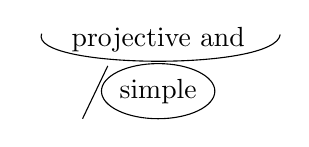
\begin{tikzpicture}
  \node[inner sep=0pt] (addition) at (0,0.65) {\inserted{projective and}};
  \node[inner sep=0pt] (simple) at (0,0) {simple};
  \handwritten{
    \draw (-1.48,0.73) .. controls (-1.65,0.28) and (1.50,0.25) .. (1.55,0.72);
    \draw (simple.center) ellipse (0.72cm and 0.35cm);
    \draw (-0.96,-0.35) -- (-0.64,0.32);
  }
\end{tikzpicture}}
\reversemarginpar
\margin{\handwritten{\figure{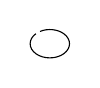
\begin{tikzpicture}\draw (-0.18,0.13) arc[start angle=135,end angle=480,x radius=0.25cm,y radius=0.18cm];\end{tikzpicture}}impossible if\\$X$ smooth !}}
\normalmarginpar
\noindent over $S$ and $X'\handwritten{\to}X$ birational,\unsure{orx|or\deleted{r}|orr} alternatively, \deleted{\unsure{if $X'$ finite}} $X$ and $X'$ projective and normal over $S$, and $f:X'\handwritten{\to}X$ finite. A counterexample in the latter case would of course provide a couterexample to the effectivity
\figure{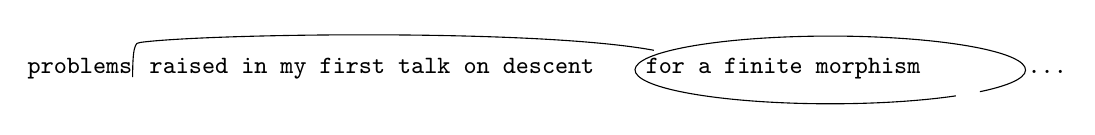
\begin{tikzpicture}[every node/.style={font=\small\ttfamily,inner sep=0pt,anchor=base west}]
  \node (problem) at (0,0) {problem\deleted{\unsure{s}}};
  % The circled phrase is attached after problem by the drawn return line.
  % It remains at its typed physical position on the right in this reproduction.
  \node (morphism) at (7.85,0) {\inserted{for a finite morphism}};
  \node (raised) at (1.55,0) {raised in my first talk on descent};
  \node at (12.70,0) {\dots};
  \handwritten{
    \draw (12.10,-0.236) arc[start angle=320,end angle=670,x radius=2.48cm,y radius=0.43cm];
    \draw (7.96,0.29) .. controls (6.45,0.57) and (2.25,0.50) .. (1.44,0.39)
      .. controls (1.37,0.40) and (1.34,0.32) .. (1.34,-0.05);
  }
\end{tikzpicture}}

``Problem A'' is the following: given $X/S$ and \deleted{any} Module $F$ on $X$, to represent the functor on the category of $S$-preschemes taking any $S'/S$ into \deleted{the empty or} into a one-element \inserted{or into the empty} set; according as to wheter $F'$ on $X'/S'$ is flat with respect to $S'$\inserted{\handwritten{or not}}, where $X'=X\mathbin{x}_S S'$, $F'=F\unsure{2|x|\otimes}_S S'$ . Given $X/S$, we say that ``Problem A \inserted{\handwritten{for $X/S$}} has always a solution'' if for every coherent $F\handwritten{'}$ on \deleted{$X$}\inserted{\handwritten{some $X'/S'$}}, the previous functor \inserted{\handwritten{on $(\mathrm{Sch})/S'$}} is representable by a \inserted{$S\handwritten{'}$\handwritten{-}}scheme of finite type. The main step in my proof of existence of Hilbert schemes shows that this condition is satisfied when $X/S$ is projective,
% archive sheet number: 77
